\documentclass[12pt]{article}
\usepackage{amsmath}
\usepackage{amssymb}
\usepackage{graphicx}
% \usepackage{physics}
\usepackage{siunitx}
\usepackage{wrapfig}

% \AtBeginDocument{\RenewCommandCopy\qty\SI}

\newcommand{\E}[1]{\times 10^{#1}}

\title{
    Chapter 20 End-of-Chapter Problems
    \\ \small
    Halliday \& Resnick, 10th Edition
}

\author{Donald Aingworth IV}

\date{\small Hit me where it Matters}

\begin{document}
    \DeclareSIUnit{\atm}{atm}
    \DeclareSIUnit{\cal}{\ cal}
    \DeclareSIUnit{\Cal}{\ Cal}
    \DeclareSIUnit{\calorie}{\ cal}
    \DeclareSIUnit{\Calorie}{\ Cal}
    \DeclareSIUnit{\celsiusdegree}{C^\circ}
    \DeclareSIUnit{\fahrenheit}{^\circ F}
    \DeclareSIUnit{\fahrenheitdegree}{F^\circ}
    \DeclareSIUnit{\torr}{\ torr}

    \maketitle

    \pagebreak
    \section{Problem 1}
        Suppose 4.00 mol of an ideal gas undergoes a reversible isothermal expansion from volume $V_1$ to volume $V_2 = 2.00\,V_1$ at temperature $T = 400\,\unit{\kelvin}$. 
        Find (a) the work done by the gas and (b) the entropy change of the gas. 
        (c) If the expansion is reversible and adiabatic instead of isothermal, what is the entropy change of the gas?

        \subsection{Solution (a)}
            The work done by a system is defined as an integral.
            \begin{equation}
                W   =   \int_{i}^{f} p\,dV
            \end{equation}

            We do not know the value of the pressure, but the ideal gas law can be used here.
            \begin{equation}
                pV = nRT \to p = \frac{nRT}{V}
            \end{equation}

            This in turn can be put into the above equation.
            Bear in mind thet the number of moles and the temperture remain constant.
            \begin{align}
                W_{\rm in}  &=  -\int_{V_i}^{V_f} \frac{nRT}{V}\,dV
                    =   -nRT\,\int_{V_i}^{2V_i} \frac{1}{V}\,dV\\
                    &=  -nRT\,\left[ \ln(V) \right]_{V_i}^{2V_i}
                    =   -nRT\ln\left( \frac{2V_i}{V_i} \right)\\
                    &=  -nRT\ln\left( 2 \right)
                    =   -4*8.31*400*\ln(2)\\
                    &=  -13296*\ln(2)
                    =   \boxed{-9216.1\,\unit{\joule}}
            \end{align}

        \subsection{Solution (b)}
            The entropy change of a system is also defined by an equation.
            \begin{equation}
                \Delta S    =   \int_{i}^{f} \frac{1}{T}\,dQ
            \end{equation}

            This is an isothermal process, so the temperature remains constant. 
            Due to that, we can simplify our equation for the change in entropy.
            \begin{align}
                \Delta S    &=  \int_{i}^{f} \frac{1}{T}\,dQ
                    =   \frac{1}{T}\int_{i}^{f} \,dQ
                    =   \frac{Q}{T}
            \end{align}

            We know the work done on the gas.
            The change in internal energy is correlated with the change in temperature ($\Delta E_{\rm int} = nC_V \Delta T$).
            Since there is no change in temperature, there would be no change in internal energy ($\Delta E_{\rm int} = 0$).
            This can be used with the first law of thermodynamics to find the heat inserted.
            \begin{eqnarray}
                \Delta E_{\rm int}  =   Q_{\rm in} + W_{\rm in}\\
                0   =   Q_{\rm in}  -   9216.1\,\unit{\joule}\\
                Q_{\rm in}  =   9216.1\,\unit{\joule}
            \end{eqnarray}

            This can be used ot find the change in entropy.
            \begin{align}
                \Delta S    &=  \frac{Q}{T}
                    =   \frac{9216.1\,\unit{\joule}}{400\unit{\kelvin}}
                    =   \boxed{23.04\,\unit{\joule/\kelvin}}
            \end{align}

        \subsection{Solution (c)}
            If the process is adiabatic, there is no net heat inserted in at all.
            This means that $Q = 0$. 
            Since the temperature is also constant, the net formula would be solvable.
            \begin{align}
                \Delta S    &=  \frac{1}{T} \int_{i}^{f}\,dQ
                    =   \frac{Q_{\rm in}}{T}
                    =   \frac{0}{T}
                    =   \boxed{0\,\unit{\joule}}
            \end{align}

    \pagebreak
    \section{Problem 3}
        A 2.50 mol sample of an ideal gas expands reversibly and isothermally at 360 K until its volume is doubled. 
        What is the increase in entropy of the gas?

        \subsection{Solution}
            The process is isothermal, so $T$ is constant, $\Delta T = 0$, and $\Delta E_{\rm int} = 0$.
            We can use this to find the work done on the gas.
            Since we are looking to double the volume, the formula for the final volume would be $V_f = 2V_i$.
            We can also use the ideal gas law here.
            \begin{gather}
                pV  =   nRT \to p = \frac{nRT}{V}\\
                \begin{align}
                    W   &=  -\int_{V_i}^{V_f} p\,dV
                        =   -\int_{V_i}^{2V_i} \frac{nRT}{V}\,dV
                        =   -nRT\int_{V_i}^{2V_i} \frac{1}{V}\,dV\\
                        &=  -nRT\left[ \ln(V) \right]_{V_i}^{2V_i}
                        =   -nRT\ln\left( \frac{2V_i}{V_i} \right)
                        =   -nRT\ln(2)
                \end{align}
            \end{gather}

            The work inserted is directly related to heat inserted, itself directly related to enchange in entropy, so we can use that.
            Bear in mind this is an isothermal process.
            \begin{gather}
                \Delta E_{\rm int}  =   0
                    =   Q + W\\
                Q   =   -W
                    =   nRT\ln(2)\\
                \begin{align}
                    \Delta S    &=  \frac{Q}{T}
                        =   \frac{nRT\ln(2)}{T}
                        =   nR\ln(2)\\
                        &=  2.50 * 8.31 * \ln(2)
                        =   \boxed{14.4\,\unit{\joule}}
                \end{align}
            \end{gather}

    \pagebreak
    \section{Problem 5}
        Find (a) the energy absorbed as heat and (b) the change in entropy of a 2.00 kg block of copper whose temperature is increased reversibly from 25.0\unit{\celsius} to 100\unit{\celsius}. 
        The specific heat of copper is 386 \unit{\joule/\kilo\gram\cdot\kelvin}.

        \subsection{Solution (a)}
            First we can calculate the change in temperature.
            \begin{equation}
                \Delta T    =   100\unit{\celsius} - 25\unit{\celsius}
                    =   75\unit{\celsiusdegree}
                    =   75\unit{\kelvin}
            \end{equation}

            Heat absorbed is calculatable from there from the change in temperature.
            \begin{equation}
                Q   =   cm\Delta T
                    =   386\,\unit{\frac{\joule}{\kilo\gram\cdot\kelvin}} * 2\,\unit{\kilo\gram} * 75\unit{\kelvin}
                    =   \boxed{57900\,\unit{\joule}}
            \end{equation}

        \subsection{Solution (b)}
        The change in entropy is calculatable by an integral.
        \begin{align}
            \Delta S    &=  \int_{i}^{f}\frac{1}{T}\,dQ
        \end{align}

        We have our known equation of the heat, which we can adapt for use differentially.
        \begin{gather}
            Q   =   cm\Delta T\\
            dQ  =   cm\,dT
        \end{gather}

        This can be put into the integral above.
        \begin{align}
            \Delta S    &=  \int_{25\unit{\kelvin}}^{75\unit{\kelvin}}\frac{cm}{T}\,dT
                =   cm \int_{25\unit{\celsius}}^{75\unit{\celsius}}\frac{1}{T}\,dT
                =   cm\ln\left( \frac{100\unit{\celsius}}{25\unit{\celsius}} \right)\\
                &=  386\,\unit{\frac{\joule}{\kilo\gram\cdot\kelvin}} * 2\,\unit{\kilo\gram} * \ln\left( \frac{373\unit{\kelvin}}{298\unit{\kelvin}} \right)\\
                &=  \boxed{173.3\,\unit{\joule/\kelvin}}
        \end{align}

    \pagebreak
    \section{Problem 7}
        A 50.0 g block of copper whose temperature is 400 K is placed in an insulating box with a 100 g block of lead whose temperature is 200 K. 
        (a) What is the equilibrium temperature of the two-block system? 
        (b) What is the change in the internal energy of the system between the initial state and the equilibrium state? 
        (c) What is the change in the entropy of the system? (See Table 18-3.)

        \subsection{Solution (a)}
            There's an equivalence statement that can be made about the heat traded between the blocks.
            \begin{gather}
                Q_{\rm net} =   0   =   Q_{\rm Cu} + Q_{\rm Pb}\\
                -Q_{\rm Cu}  =   Q_{\rm Pb}\\
                -c_{\rm Cu} m_{\rm Cu} \Delta T_{\rm Cu} = c_{\rm Pb} m_{\rm Pb} \Delta T_{\rm Pb} \\
                386\,\unit{\frac{J}{\kilo\gram\cdot\kelvin}} * 0.05\,\unit{\kilo\gram} * \left( 400\unit{\kelvin} - T_f \right) = 128\,\unit{\frac{J}{\kilo\gram\cdot\kelvin}} * 0.1\,\unit{\kilo\gram} * \left( T_f - 200\unit{\kelvin} \right)\\
                19.3\,\unit{\joule/\kelvin} * 400\unit{\kelvin} - 19.3\,\unit{\joule/\kelvin} * T_f = 12.8\,\unit{\joule/\kelvin} * T_f - 12.8\,\unit{\joule/\kelvin} * 200\unit{\kelvin}\\
                T_f * (19.3\,\unit{\joule/\kelvin} + 12.8\,\unit{\joule/\kelvin}) = 19.3\,\unit{\joule/\kelvin} * 400\unit{\kelvin} + 12.8\,\unit{\joule/\kelvin} * 200\unit{\kelvin}\\
                32.1\,\unit{\joule/\kelvin} * T_f = 7720\,\unit{\joule} + 2560\,\unit{\joule}
                    =   10280\,\unit{\joule}\\
                T_f =   \frac{10280\,\unit{\joule}}{32.1\,\unit{\joule/\kelvin}}
                    =   \boxed{320\unit{\kelvin}}
            \end{gather}

        \subsection{Solution (b)}
            Since the system is insulated, all the energy that goes out of one of the blocks goes into the other. 
            This makes there no net change in the net energy overall.
            The answer is \boxed{0}.

        \subsection{Solution (c)}
            This can be found by an integral, but first we should change a known equation (for the heat) into a differential one.
            For this, we can use our earlier equation for the heat. 
            \begin{align}
                Q   &=  cm\Delta T\\
                dQ  &=  cm\,dT\\
                Q_{\rm net} &=  Q_{\rm Cu} + Q_{\rm Pb}\\
                dQ_{\rm net}    &=  dQ_{\rm Cu} + dQ_{\rm Pb}\\
                    &=  c_{\rm Cu} m_{\rm Cu} \, dT_{\rm Cu} + c_{\rm Pb} m_{\rm Pb} \, dT_{\rm Pb}
            \end{align}

            At this point, we can put this into the integral of the change in entropy.
            \begin{align}
                \Delta S    &=  \int \frac{1}{T}\,dQ
                    =   \int_{400\unit{\kelvin}}^{320\unit{\kelvin}} \frac{c_{\rm Cu} m_{\rm Cu}}{T} \,dT + \int_{200\unit{\kelvin}}^{320\unit{\kelvin}} \frac{c_{\rm Pb} m_{\rm Pb}}{T} \,dT\\
                    &=  c_{\rm Cu} m_{\rm Cu} \left[ \ln(T) \right]_{400\unit{\kelvin}}^{320\unit{\kelvin}} + c_{\rm Pb} m_{\rm Pb} \left[ \ln(T) \right]_{200\unit{\kelvin}}^{320\unit{\kelvin}}\\
                    &=  c_{\rm Cu} m_{\rm Cu} \ln\left( \frac{320}{400} \right) + c_{\rm Pb} m_{\rm Pb} \ln\left( \frac{320}{200} \right)\\
                    &=  386\,\unit{\frac{\joule}{\kilo\gram\cdot\kelvin}} * 0.05\,\unit{\kilo\gram} * \ln\left( \frac{320}{400} \right) + 128\,\unit{\frac{\joule}{\kilo\gram\cdot\kelvin}} * 0.1\,\unit{\kilo\gram} * \ln\left( \frac{320}{200} \right)\\
                    &=  19.3 * \ln(0.8) + 12.8 * \ln(1.6)
                    =   \boxed{1.709\,\unit{\joule/\kelvin}}
            \end{align}

    \pagebreak
    \section{Problem 9}
        A 10 g ice cube at -10\unit{\celsius} is placed in a lake whose temperature is 15°C. 
        Calculate the change in entropy of the cube-lake system as the ice cube comes to thermal equilibrium with the lake. 
        The specific heat of ice is 2220 \unit{\joule/\kilo\gram\cdot\kelvin}. 
        (Hint: Will the ice cube affect the lake temperature?)

        \subsection{Solution}
            We can assume that the ice will only negligibly affect the lake's temperature.
            From this, we can devise the formula for the energy used to melt and warm up the ice.
            \begin{align}
                Q   &=  c_{\rm ice} m \Delta T_1 + L_{\rm fus} m + c_{\rm water} m \Delta T_2\\
                    &=  2220 * 0.010 * (10\,\unit{\kelvin}) + 334 * 10 + 4186 * 0.010 * (15\,\unit{\kelvin})\\
                    &=  222 + 3340 + 627.9
                    =   4189.9\,\unit{\joule}
            \end{align}

            This is the total heat required for the entire block of ice to melt and warm.
            We can turn this differentiable, with respect to the temperature when warming and with respect to the mass when melting.
            \begin{align}
                dQ  &=  c_{\rm ice} m\,dT + L_{\rm fus}\,dm + c_{\rm water} m\,dT
            \end{align}

            We can from here find the change in entropy by integral.
            The heat from fusion will be from 0g to 10g rather than from 10g to 0g because it is measuring the mass converted to water rather than the mass that is ice.
            \begin{align}
                \Delta S    &=  \int_{i}^{f}\frac{1}{T}\,dQ
                    =   \int_{263\unit{\kelvin}}^{273\unit{\kelvin}} \frac{c_{\rm ice} m}{T}\,dT
                        +   \int_{0\unit{\gram}}^{10\unit{\gram}} L_{\rm fus}\,dm
                        +   \int_{273\unit{\kelvin}}^{288\unit{\kelvin}} \frac{c_{\rm water} m}{T}\,dT\\
                    &=  c_{\rm ice} m\,\left[ \ln(T) \right]_{263\unit{\kelvin}}^{273\unit{\kelvin}} + L_{\rm fus}\,\left[ m \right]_{0\unit{\gram}}^{10\unit{\gram}} + c_{\rm ice} m\,\left[ \ln(T) \right]_{273\unit{\kelvin}}^{288\unit{\kelvin}}\\
                    &=  2220 * 0.010 * \ln\left( \frac{273}{263} \right) + \frac{334 * 10}{273} + 4186 * 0.010 * \ln\left( \frac{288}{273} \right)\\
                    &=  0.828\,\unit{\joule/\kelvin} + 12.234\,\unit{\joule/\kelvin} + 2.239\,\unit{\joule/\kelvin}
                    =   15.302\,\unit{\joule/\kelvin}
            \end{align}

            The lake also releases heat, which would itself give a change in entropy. 
            Since the lake's temperature is nearly constant, the process is isothermal.
            \begin{align}
                \Delta S    &=  \frac{Q}{T}
                    =   \frac{-4189.9\,\unit{\joule}}{288}
                    =   -14.548\,\unit{\joule/\kelvin}
            \end{align}

            Add the two changes in entropy together to find the ultimate change in entropy.
            \begin{align}
                \Delta S_{\Sigma}   &=  15.302\,\unit{\joule/\kelvin} - 14.548\unit{\joule/\kelvin}
                    =   \boxed{0.754\,\unit{\joule/\kelvin}}
            \end{align}

    \pagebreak
    \section{Problem 15}
        A mixture of 1773 g of water and 227 g of ice is in an initial equilibrium state at 0.000\unit{\celsius}. 
        The mixture is then, in a reversible process, brought to a second equilibrium state where the water-ice ratio, by mass, is 1.00 : 1.00 at 0.000\unit{\celsius}. 
        (a) Calculate the entropy change of the system during this process. 
        (The heat of fusion for water is 333 kJ/kg.) 
        (b) The system is then returned to the initial equilibrium state in an irreversible process (say, by using a Bunsen burner). 
        Calculate the entropy change of the system during this process. 
        (c) Are your answers consistent with the second law of thermodynamics?

        \subsection{Solution (a)}
            Mass is constant, so the total mass of the water and ice will be equal, itself the average of the total massses of ice and water.
            \begin{align}
                m_f &=  \frac{1773\,\unit{\gram} + 227\,\unit{\gram}}{2}
                    =   \frac{2000}{2}\,\unit{\gram}
                    =   1\,\unit{\kilo\gram}
            \end{align}

            That's a convenient value to use.
            We have an equation of the energy (heat in this case) used in fusion. 
            There is more water than ice here, so the energy would be causing water would be turning into ice.
            \begin{align}
                \Delta m    &=  m_f - m_i
                    =   1.000\,\unit{\kilo\gram} - 1.773\,\unit{\kilo\gram}
                    =   -0.773\,\unit{\kilo\gram}\\
                Q   &=  L_V m
                    =   333\,\unit{\joule/\gram} * (-773\,\unit{\gram})
                    =   -257409\,\unit{\joule}
            \end{align}

            This can in turn be used in the calculation of change of entropy.
            \begin{align}
                \Delta S    &=  \frac{Q}{T}
                    =   \frac{-257409\,\unit{\joule}}{273\unit{\kelvin}}
                    =   \boxed{-942\,\unit{\joule/\kelvin}}
            \end{align}

            The second law of thermodynamics seems to contradict this, with $\Delta S < 0$ being impossible.
            However, that only applies to closed systems, while this is not a closed system.

        \subsection{Solution (b)}
            The process would be of equal heat and opposite heat to the reversible process.
            Since the temperature would remain constant, the change in entropy would be equal and opposite as well.
            \begin{equation}
                \Delta S    =   \boxed{942\,\unit{\joule/\kelvin}}
            \end{equation}

        \subsection{Solution (c)}
            This would not be inconsistent with the second law of thermodynamics, so the answer is \boxed{yes}.
            As stated before, this would be an open system, or at least there is nothing saying it is not.

    \pagebreak
    \section{Problem 23}
        A Carnot engine whose low-temperature reservoir is at 17\unit{\celsius} has an efficiency of 40\%. 
        By how much should the temperature of the high-temperature reservoir be increased to increase the efficiency to 50\%?

        \subsection{Solution}
            First we convert temperature from Celsius to Kelvin.
            \begin{equation}
                17\unit{\celsius} + 273.15\unit{\kelvin} = 290.15\unit{\kelvin}
            \end{equation}

            This gives us the low temperature and we already know the efficiency. 
            We can also calculate the high temperature.
            \begin{gather}
                \varepsilon_C   =   1 - \frac{T_L}{T_H}\\
                \frac{T_L}{T_H} =   1 - \varepsilon_C\\
                \begin{align}
                    T_{H;i} &=  \frac{T_L}{1 - \varepsilon_C}
                        =   \frac{290.15\unit{\kelvin}}{1 - 0.4}
                        =   \frac{290.15\unit{\kelvin}}{0.60}
                        =   483.583\unit{\kelvin}\\
                    T_{H;f} &=  \frac{T_L}{1 - \varepsilon_C}
                        =   \frac{290.15\unit{\kelvin}}{1 - 0.5}
                        =   \frac{290.15\unit{\kelvin}}{0.5}
                        =   580.3\unit{\kelvin}\\
                    \Delta T_H  &=  580.3\unit{\kelvin} - 483.583\unit{\kelvin}
                        =   \boxed{96.717\unit{\kelvin}}
                \end{align}
            \end{gather}

    \pagebreak
    \section{Problem 25}
        A Carnot engine has an efficiency of 22.0\%. 
        It operates between constant-temperature reservoirs differing in temperature by 75.0 \unit{\celsiusdegree}. 
        What is the temperature of the (a) lower-temperature and (b) higher-temperature reservoir?

        \subsection{Solution (a)}
            Start by finding the ratio of the hot and cold temperatures.
            \begin{gather}
                \varepsilon_C   =   1 - \frac{T_L}{T_H}\\
                \begin{align}
                    \frac{T_L}{T_H} &=  1 - \varepsilon_C
                        =   1 - 0.22
                        =   0.78
                \end{align}\\
                T_L =   0.78\,T_H
            \end{gather}

            From here, we can put this into the change in temperature $\Delta T$.
            \begin{gather}
                \begin{align}
                    \Delta T    &=  75\,\unit{\celsiusdegree}
                        =   \left| T_L - T_H \right|
                        =   \left| (0.78 - 1)T_H \right|
                        =   0.22\,T_H
                \end{align}\\
                T_H =   \frac{75\unit{\kelvin}}{0.22}
                    =   340.91\unit{\kelvin}\\
                T_L =   0.78\,T_H
                    =   0.78 * 340.91\unit{\kelvin}
                    =   \boxed{265.91\unit{\kelvin}}
            \end{gather}

        \subsection{Solution (b)}
            As found in my solution to part (a), the temperature is \boxed{265.91\unit{\kelvin}}.

    \pagebreak
    \section{Problem 27}
        A Carnot engine operates between 235\unit{\celsius} and 115\unit{\celsius}, absorbing $6.30\E{4}$ J per cycle at the higher temperature.
        (a) What is the efficiency of the engine? 
        (b) How much work per cycle is this engine capable of performing?

        \subsection{Solution (a)}
            We start with an equation for the efficiency.
            \begin{gather}
                e_C =   1 - \frac{T_L}{T_H}
                    =   \frac{\left| W \right|}{\left| Q_H \right|}
            \end{gather}

            We also can convert the temperatures from Celsius into Kelvin.
            \begin{align}
                T_C &=  115\unit{\celsius} + 273.15\unit{\kelvin}
                    =   388.15\unit{\kelvin}\\
                T_H &=  235\unit{\celsius} + 273.15\unit{\kelvin}
                    =   508.15\unit{\kelvin}
            \end{align}

            These can be used to find the efficiency of the carnot engine.
            \begin{align}
                e_C &=  1 - \frac{T_L}{T_H}
                    =   1 - \frac{388.15}{508.15}\\
                    &=  1 - 0.7638492571
                    =   \boxed{0.2361507429}
            \end{align}

    \pagebreak
    \section{Problem 29}
        \begin{wrapfigure}{r}{0.25\textwidth}
            \vspace{-30pt}
            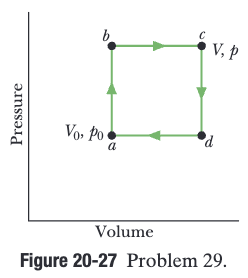
\includegraphics[width=0.25\textwidth]{picture_20-27.png} 
            % \label{fig:wrapfig}
        \end{wrapfigure}
        Figure 20-27 shows a reversible cycle through which 1.00 mol of a monatomic ideal gas is taken. 
        Assume that $p = 2p_0$, $V = 2V_0$, $p_0 = 1.01 \E{5}$ Pa, and $V_0 = 0.0225 \unit{\meter^3}$. 
        Calculate (a) the work done during the cycle, (b) the energy added as heat during stroke $abc$, and (c) the efficiency of the cycle. 
        (d) What is the efficiency of a Carnot engine operating between the highest and lowest temperatures that occur in the cycle? 
        (e) Is this greater than or less than the efficiency calculated in (c)?

        \subsection{Solution (a)}
            There are four processes, two isobaric and two isochoric.
            We can calculate the work done in each process and add these together to find the total work done on the gas during the cycle.
            \begin{align}
                W_{ab}  &=  0\\
                W_{bc}  &=  -p\Delta V
                    =   -2p_0 (2V_0 - V_0)
                    =   -2p_0 V_0\\
                W_{cd}  &=  0\\
                +\,\,\,\,\,\,
                W_{da}    &=  -p\Delta V
                    =   -p_0 (V_0 - 2V_0)
                    =   p_0 V_0\\
                \hline
                W   =   \int_{i}^{f} p\,dV
                    &=  -p_0 V_0
                    =   -1.01\E{5}\,\unit{\pascal} * 0.0225\,\unit{\meter^3}
                    =   \boxed{-2272.5\,\unit{joule}}
            \end{align} 

        \subsection{Solution (b)}
            The ideal gas law and equation for the work can be used here.
            \begin{align}
                \Delta E_{\rm int}  &=  nC_V\,\Delta T
                    =   \frac{3}{2} \times nR\,\Delta T
            \end{align}

            Using the ideal gas law, we can find the initial and final temperatures.
            \begin{gather}
                pV  =   nRT \to
                T   =   \frac{pV}{nR}\\
                T_i =   \frac{p_i V_i}{nR}
                    =   \frac{1.01 \E{5} * 0.0225}{1 * 8.31}
                    =   273.46\,\unit{\kelvin}
            \end{gather}
            \begin{gather}
                T_f =   \frac{p_f V_f}{nR}
                    =   \frac{2.02 \E{5} * 0.0450}{1 * 8.31}
                    =   1093.86\,\unit{\kelvin}\\
                \Delta T    =   T_f - T_i
                    =   820.40\,\unit{\kelvin}
            \end{gather}

            This in turn allows us to find the total change in internal energy using the above equation.
            \begin{align}
                \Delta E_{\rm int}  &=  \frac{3}{2} \times nR\,\Delta T
                    =   \frac{3}{2} \times 1\,\unit{\mole} * 8.31 * 820.40\,\unit{\kelvin}
                    =  10226.25\,\unit{\joule}
            \end{align}

            From here, we can find the work done along $abc$. 
            We have most of the informatin for this from part (a).
            \begin{align}
                W_{\rm abc} &=  W_{\rm ab} + W_{\rm bc}
                    =   0 - 2 p_0 V_0\\
                    &=  -2 * 1.01\E{5} * 0.0225
                    =   -4545\,\unit{\joule}
            \end{align}
            
            From here, we use the first law of thermodynamics.
            \begin{gather}
                \Delta E_{\rm int} = Q + W\\
                \begin{align}
                    Q   &=  \Delta E_{\rm int} - W
                        =   10226.25\,\unit{\joule} + 4545\,\unit{\joule}\\
                        &=  \boxed{14771.25\,\unit{\joule}}
                \end{align}
            \end{gather}

        \subsection{Solution (c)}
            The efficiency of an engine is equal to the ratio of the absolute value of the heat inserted to the work inserted.
            Our answer in (b) would be the heat, while our answer in (a) would be the work, taking the absolute value in both cases.
            \begin{align}
                \varepsilon &=  \frac{| W |}{| Q_H |}
                    =   \frac{2272.5\,\unit{joule}}{14771.25\,\unit{\joule}}
                    =   0.1538
                    =   \boxed{15.38\%}
            \end{align}

        \subsection{Solution (d)}
            There is a formula for the efficiency of a carnot engine.
            \begin{align}
                \varepsilon_C   &=  1 - \frac{Q_L}{Q_H}
                    =   1 - \frac{273.46\,\unit{\kelvin}}{1093.86\,\unit{\kelvin}}
                    =   \frac{820.40\,\unit{\kelvin}}{1093.86\,\unit{\kelvin}}
                    =   \boxed{0.75}
            \end{align}

        \subsection{Solution (e)}
            The Carnot engine being a perfect kind of engine, the efficiency would be \boxed{greater}. 

    \pagebreak
    \section{Problem 37}
        A heat pump is used to heat a building. 
        The external temperature is less than the internal temperature. 
        The pump's coefficient of performance is 3.8, and the heat pump delivers 7.54 MJ as heat to the building each hour. 
        If the heat pump is a Carnot engine working in reverse, at what rate must work be done to run it?

        \subsection{Solution}
            We have the coefficient of performance and the heat inserted into the house.
            From this, we can calculate the low power.
            \begin{gather}
                K_C =   \frac{| Q_L |}{| Q_H | - | Q_L |}
                    =   \frac{| Q_L |}{| W |}\\
                \frac{1}{K_C}   =   \frac{| Q_H |}{| Q_L |} - 1\\
                \frac{K_C + 1}{K_C} =   \frac{| Q_H |}{| Q_L |}\\
                \frac{K_C + 1}{K_C * | Q_H |} =   \frac{1}{| Q_L |}\\
                | Q_L | =   \frac{K_C * | Q_H |}{K_C + 1}\\
                | P_L | =   \frac{K_C * | P_H |}{K_C + 1}
                    =   \frac{3.8 * 7.54\,\unit{\mega\joule/\hour}}{4.8}
                    =   5.97\,\unit{\mega\joule/\hour}\\
                |W| =   |Q_H| - |Q_L|
                    =   7.54\E{6} - 5.97\E{6}
                    =   1.57\E{6}\,\unit{\joule}\\
                |P| =   \frac{1.57\E{6}\,\unit{\joule}}{1\,\unit{\hour}}
                    =   \frac{1.57\E{6}\,\unit{\joule}}{3600\,\unit{\second}}
                    =   \boxed{436\,\unit{\watt}}
            \end{gather}

            I'm kind of questioning the answer to this. 

    \pagebreak
    \section{Problem 39}
        A Carnot air conditioner takes energy from the thermal energy of a room at 70\unit{\fahrenheit} and transfers it as heat to the outdoors, which is at 96\unit{\fahrenheit}. 
        For each joule of electric energy required to operate the air conditioner, how many joules are removed from the room?

        \subsection{Solution}
            The first thing we do is convert the Fahrenheit temperatures into Celsius.
            \begin{align}
                T_{\unit{\celsius}}  &=  \frac{5}{9}(T_{\unit{\fahrenheit}} - 32\unit{\fahrenheitdegree})\,\unit{\celsius}\\
                T_L &=  70\unit{\fahrenheit}
                    =   \frac{5}{9}(70\unit{\fahrenheit} - 32\unit{\fahrenheitdegree})\,\unit{\celsius}
                    =   \frac{5}{9} * 38\unit{\celsius} 
                    =   21.11\unit{\celsius}\\
                T_H &=  96\unit{\fahrenheit}
                    =   \frac{5}{9}(96\unit{\fahrenheit} - 32\unit{\fahrenheitdegree})\,\unit{\celsius}
                    =   \frac{5}{9} * 64\unit{\celsius}
                    =   35.56\unit{\celsius}
            \end{align}

            Next, we convert Celsius to Kelvin.
            \begin{align}
                T_{\unit{\kelvin}}  &=  T_{\unit{\celsius}} + 273.15\unit{\kelvin}\\
                T_L &=  21.11\unit{\celsius} + 273.15\unit{\kelvin}
                    =   294.26\unit{\kelvin}\\
                T_H &=  35.56\unit{\celsius} + 273.15\unit{\kelvin}
                    =   308.71\unit{\kelvin}
            \end{align}

            From here, we can find the Carnot coefficient of performance of the air conditioner (a Carnot refrigerator).
            \begin{align}
                K_C &=  \frac{T_L}{T_H - T_L}
                    =   \frac{294.26\unit{\kelvin}}{308.71\unit{\kelvin} - 294.26\unit{\kelvin}}
                    =   \frac{294.26}{14.45}
                    =   20.36
            \end{align}

            This in turn is still a refrigerator, which is a ratio of the heat removed to the work needed to be done.
            The work in this case would technically be only one joule.
            \begin{gather}
                K_C =   \frac{|Q_L|}{|W|}
                    =   \frac{|Q_L|}{1\unit{\joule}}
                    =   20.36\\
                Q_L =   \boxed{20.36\unit{\joule}}
            \end{gather}

    \pagebreak
    \section{Problem 43}
        \begin{wrapfigure}{r}{0.25\textwidth}
            \vspace{-30pt}
            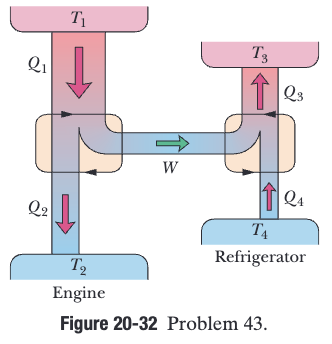
\includegraphics[width=0.25\textwidth]{picture_20-32.png} 
            % \label{fig:wrapfig}
        \end{wrapfigure}
        Figure 20-32 represents a Carnot engine that works between temperatures $T_1$ = 400 K and $T_2$ = 150 K and drives a Carnot refrigerator that works between temperatures $T_3$ = 325 K and $T_4$ = 225 K. 
        What is the ratio $Q_3/Q_1$?

        \subsection{Solution}
            We have some equations related to $Q_1$ and $Q_3$. 
            \begin{gather}
                \frac{W}{Q_1} = \varepsilon_C = 1 - \frac{T_2}{T_1} \to
                Q_1 = W \frac{T_1}{T_1 - T_2}\\
                \frac{Q_4}{W} = K_C = \frac{T_4}{T_3 - T_4} = \frac{Q_4}{Q_3 - Q_4}\\
                \frac{W}{Q_4} = \frac{T_3 - T_4}{T_4} = \frac{Q_3 - Q_4}{Q_4}\\
                Q_3 = Q_4 + W \leftrightarrow Q_4 = Q_3 - W\\
                Q_3 = W \left( \frac{T_4}{T_3 - T_4} + 1 \right)
                    =   W \frac{T_3}{T_3 - T_4}
            \end{gather}

            From here, we can calculate the fraction of $\frac{Q_3}{Q_1}$.
            \begin{align}
                \frac{Q_3}{Q_1} &=  \frac{W \frac{T_3}{T_3 - T_4}}{W \frac{T_1}{T_1 - T_2}}
                    =   \frac{T_3}{T_3 - T_4} * \frac{T_1 - T_2}{T_1}
                    =   \frac{325\unit{\kelvin} * (400\unit{\kelvin} - 150\unit{\kelvin})}{400\unit{\kelvin} * (325\unit{\kelvin} - 225\unit{\kelvin})}\\
                    &=  \frac{325\unit{\kelvin} * 250\unit{\kelvin}}{400\unit{\kelvin} * 100\unit{\kelvin}}
                    =   \frac{81250}{40000}
                    =   \frac{65}{32}
                    =   \boxed{2.03125}
            \end{align}

    \pagebreak
    \section{Problem 45}
        Construct a table like Table 20-1 for eight molecules.

        \subsection{Solution}
        {\small \begin{tabular}{ r r r r l l }
            \multicolumn{3}{c}{Configuration}   & Multiplicity W    & Calculation of W  & Entropy ($10^{-23} \unit{\joule/\kelvin}$)\\
            Label   &   $n_1$   &   $n_2$       & \# of microstates & (Eq'n 20-20)      & (Eq'n 20-21)\\
            \hline
            I   &   8   &   0   &   1   &   $\frac{N!}{n_1! n_2!} = \frac{8!}{8! 0!} = 1$   &   0
            \\
            II  &   7   &   1   &   8   &   $\frac{N!}{n_1! n_2!} = \frac{8!}{7! 1!} = 8$   &   2.87
            \\
            III &   6   &   2   &   28  &   $\frac{N!}{n_1! n_2!} = \frac{8!}{6! 2!} = 28$  &   4.60
            \\
            IV  &   5   &   3   &   56  &   $\frac{N!}{n_1! n_2!} = \frac{8!}{5! 3!} = 56$  &   5.55
            \\
            V   &   4   &   4   &   70  &   $\frac{N!}{n_1! n_2!} = \frac{8!}{4! 4!} = 70$  &   5.86
            \\
            VI  &   3   &   5   &   56  &   $\frac{N!}{n_1! n_2!} = \frac{8!}{3! 5!} = 56$  &   5.55
            \\
            VII &   2   &   6   &   28  &   $\frac{N!}{n_1! n_2!} = \frac{8!}{2! 6!} = 28$  &   4.60
            \\
            VIII&   1   &   7   &   8   &   $\frac{N!}{n_1! n_2!} = \frac{8!}{1! 7!} = 8$   &   2.87
            \\
            IX  &   0   &   8   &   1   &   $\frac{N!}{n_1! n_2!} = \frac{8!}{0! 8!} = 1$   &   0
            \\
            &&& $\overline{256}$
        \end{tabular}}

    \pagebreak
    \section{Problem 49}
        A cylindrical copper rod of length 1.50 m and radius 2.00 cm is insulated to prevent heat loss through its curved surface. 
        One end is attached to a thermal reservoir fixed at 300\unit{\celsius}; the other is attached to a thermal reservoir fixed at 30.0\unit{\celsius}. 
        What is the rate at which entropy increases for the rod-reservoirs system?

        \subsection{Solution}
            The thermal reservoirs can be assumed to have constant temperature. 
            % The rod is made of copper, so the specific heat is $386\,\unit{\frac{\joule}{\kilo\gram\cdot\kelvin}}$. 
            We have a formula for the heat that goes from the hot to the cold per unit time, which can be used here, and a formula for the change in entropy.
            \begin{gather}
                \Delta S    =   \int_{i}^{f} \frac{1}{T}\,dQ\\
                \frac{Q}{t} =   \frac{kA}{L}\Delta T
            \end{gather}

            The two heat reservoirs have constant temperatures, so we can consider their processes isothermal.
            This allows us a formula for the heat.
            \begin{align}
                \Delta S    &=  \frac{Q}{T}
            \end{align}

            Divide both sides by the unit time to get the formula for the change in entropy over time, which we can substitute our equation for the heat over time into.
            \begin{equation}
                \frac{\Delta S}{t}  =   \frac{1}{T} * \frac{Q}{t}
                    =   \frac{1}{T} * \frac{kA}{L}\Delta T
            \end{equation}

            This gives us the change in entropy over time for individual reservoirs.
            Adding the changes in entropies of the individual reservoirs together, we can get the total change in entropy.
            The entropy of the hotter system would be decreasing, while that of the colder system would be increasing.
            This in turn can be substituted in and solved.
            \begin{align}
                \frac{\Delta S}{t}  &=  \frac{kA}{L}\Delta T\,\left( \frac{1}{T_C} - \frac{1}{T_H} \right)\\
                    &=  \frac{401 * \pi (20\E{-3})^2}{1.5}*270\unit{\kelvin}\,\left( \frac{1}{303.15\unit{\kelvin}} - \frac{1}{573.15\unit{\kelvin}} \right)\\
                    &=  90.704 * 1.55\E{-3}
                    =   \boxed{0.141\,\unit{\joule/\kelvin\cdot\second}}
            \end{align}

    \pagebreak
    \section{Problem 53}
        Suppose that a deep shaft were drilled in Earth's crust near one of the poles, where the surface temperature is -40\unit{\celsius}, to a depth where the temperature is 800°C. 
        (a) What is the theoretical limit to the efficiency of an engine operating between these temperatures?
        (b) If all the energy released as heat into the low-temperature reservoir were used to melt ice that was initially at -40\unit{\celsius}, at what rate could liquid water at 0\unit{\celsius} be produced by a 100 MW power plant (treat it as an engine)? 
        The specific heat of ice is 2220 \unit{\joule/\kilo\gram\cdot\kelvin}; water's heat of fusion is 333 \unit{\kilo\joule/\kilo\gram}. 
        (Note that the engine can operate only between 0\unit{\celsius} and 800\unit{\celsius} in this case. 
        Energy exhausted at -40\unit{\celsius} cannot warm anything above -40\unit{\celsius}.)

        \subsection{Solution (a)}
            For maximum efficiency, this would have to be a Carnot engine, and as such would have a calculatable (Carnot) efficiency. 
            \begin{align}
                \varepsilon_C   &=  1 - \frac{T_L}{T_H}
                    =   1 - \frac{233.15}{1073.15}
                    =   1 - 0.21726
                    =   \boxed{0.783}
            \end{align}

        \subsection{Solution (b)}

    % \pagebreak
    \section{Problem 57}
        The temperature of 1.00 mol of a monatomic ideal gas is raised reversibly from 300 K to 400 K, with its volume kept constant. 
        What is the entropy change of the gas?

        \subsection{Solution}

    % \pagebreak
    \section{Problem 67}
        Suppose that 260 J is conducted from a constant-temperature reservoir at 400 K to one at (a) 100 K, (b) 200 K, (c) 300 K, and (d) 360 K. 
        What is the net change in entropy $\Delta S_{\rm net}$ of the reservoirs in each case? 
        (e) As the temperature difference of the two reservoirs decreases, does $\Delta S_{\rm net}$ increase, decrease, or remain the same?

        \subsection{Solution}

    % \pagebreak
    \section{Problem 71}
        A box contains N molecules. 
        Consider two configurations: configuration A with an equal division of the molecules between the two halves of the box, and configuration B with 60.0\% of the molecules in the left half of the box and 40.0\% in the right half. 
        For N = 50, what are (a) the multiplicity $W_A$ of configuration A, (b) the multiplicity $W_B$ of configuration B, and (c) the ratio $f_{B/A}$ of the time the system spends in configuration B to the time it spends in configuration A? 
        For N = 100, what are (d) $W_A$, (e) $W_B$, and (f) $f_{B/A}$? 
        For N = 200, what are (g) $W_A$, (h) $W_B$, and (i) $f_{B/A}$? 
        (j) With increasing N, does $f$ increase, decrease, or remain the same?

        \subsection{Solution}

    \pagebreak

    \tableofcontents

\end{document}